\textit{Этот билет основан на нашей офлайн лекции 2020 и видеолекции 2016}
\hyperref{https://yadi.sk/i/VhIMQ5NKq3r2v}{}{}{\textit{(cсылка)}}
\\
$$f(x) \rightarrow \underset{x\in \mathbb{R}^n}{min}$$

Данную задачу хорошо решает метод Ньютона. Но у него стоимость по памяти $O(n^2)$. Если $n > 5000$ уже просто не сможем хранить гессиан в памяти.

Первый способ обойти проблему -- CG. Но там скорость сходимости линейная. Попробуем сделать линейную стоимость по памяти и суперлинейную скорость сходимости. Начнем с обычного метода Ньютона:
$$
x_{k+1} = x_k + \alpha_k d_k
$$
\begin{align}
    H_k d_k &= -\nabla f(x) \tag{1}
\end{align}

где $H_k$ - гессиан на шаге $k$.

\noindent \textbf{Ключевая идея HFN}: решать СЛАУ(1) с помошью метода сопряженных градиентов.

Важные моменты:

\ \ 1) Вместо хранения $H$ используем процедуру "$H\cdot d$"

\ \ 2) Решаем СЛАУ неточно

1) будет обсуждаться далее (см. разностное дифферернцирование). Интуиция для 2): вдалеке от точки оптимума можно решать систему не точно, а по мере блиближения увеличивать точность.

\noindent Новый метод останова для CG:
\begin{gather*}
    r_k := H_k d_k + \nabla f_k\\
    \| r_k\| \le \eta_k\|\nabla f(x_k)\|\\
\end{gather*}

$\eta_k \in (0, 1)$ и называется \textit{форсирующей последовательностью}.
\\

\noindent \textbf{--- Локальная сходимость HFN.}

\textit{Доказательство с лекции 2020, более подробная версия в [12] раздел 7.1, теорема 7.1}

Я не уверен, что его будут требовать, его так скомканно и давали:

\begin{gather*}
    f \in C^{2, 2}_M,\ \alpha_k=1,\ g_k = \nabla f(x_k)\\
    x_{k+1} = x_k + \alpha_k d_k\\
\end{gather*}
\begin{align}
    r_k = H_k d_k + g_k \Rightarrow d_k = H_k^{-1}(r_k - g_k) \tag{2}
\end{align}
\begin{align}
    \|r_k\| \le \eta_k\|g_k\| \tag{3}
\end{align}
Покажем сходимость:
\begin{gather*}
    \|x_{k+1} - x_{\text{opt}}\| = \|x_k - x_{\text{opt}} + \underbrace{H_k^{-1}(r_k-g_k)}_{d_k \text{ по } (2)}\| \overset{\cdot H_k^{-1}}{\le} \underbrace{\|H_k^{-1}\|}_{\le\text{ const}}\cdot\|H_k(x_k - x_{\text{opt}}) - g_k + r_k\| \le\\
    \le \text{const}\cdot\big(\underbrace{\|H_k(x_k - x_{\text{opt}}) - g_k\|}_{O(\|x_k - x_{\text{opt}}\|^2)}\ \  + \underbrace{\|r_k\|}_{\le\eta_k \|g_k\| \text{ по } (3)}\big)  \le \text{const}\cdot(O(\|x_k-x_{\text{opt}}\|^2) + \eta_k\|g_k\|)\\
    \bigg\{\|g_k\| = \|\nabla f(x_k) - \underbrace{\nabla f(x_{\text{opt}})}_{0}\| \overset{\text{липш. } ?}{=} O(\|x_k - x_{\text{opt}}\|) \bigg\}\\
    \le \text{const}\cdot \left(O(\|x_k - x_{\text{opt}}\|^2) + \eta_k O(\|x_k - x_{\text{opt}}\|)\right)
    \qed\\
\end{gather*}



\noindent \textbf{--- Локальная скорость сходимости HFN.}
$$f \in C^{2, 2}_M, \alpha_k = 1. \ \ \ \ \ \ \ \ \ \|r_k\| \le \eta_k\|\nabla f(x_k)\|$$
1) $\eta_k = \eta < 1 \longrightarrow $ линейная скорость сходимости
\\
\ \ 2) $\eta_k \underset{k\rightarrow \infty}{\rightarrow} 0 \longrightarrow$ суперлинейная скорость сходимости. Обычно берут: $\eta_k=\min{\left(\dfrac{1}{2},\  \sqrt{\|\nabla f(x_k)\|}\right)}$
\\
\ \ 3) $\eta_k = O(\|\nabla f(x_k)\|) \longrightarrow$  квадратичная скорость сходимости. Обычно берут: $\eta_k=\min{\left(\dfrac{1}{2},\  \|\nabla f(x_k)\|\right)}$

\noindent Для 2) и 3) мы берем бОльшую точность для CG, он делает больше шагов, но из-за этого получаем лучшую скорость сходимости метода Ньютона. В реализации используется 2) потому что суперлинейной скорости сходимости на практике достаточно!

\textbf{Общая схема метода выглядит HFN так}:

Краткое описание дальнейшей процедуры: внутренний цикл - CG, $\{z_j\}$ играют роль $\{x_j\}$ для внутреннего запуска CG:

\begin{algorithm}[H]
    \begin{algorithmic}[1]
        \Procedure{HFN}{$f, \varepsilon, x_0$}
            \State get $\nabla f(x_0)$
            \For{$k=0, 1, 2, ...$}
                \State $\varepsilon_k \gets \min\left(\frac{1}{2},\ \sqrt{\|\nabla f_k\|}\right)\cdot\|\nabla f_k\|$
                \State $z_0=0,\ g_0=H_k z_0 + \nabla f_0,\ d_0=-g_0$
                \For{$j=0, 1, 2 ...$}
                    \State $\alpha_j \gets \dfrac{g_j^ Tg_j}{d_j^T H_j d_j}$
                    \State $z_{j+1} \gets z_j + \alpha_j d_j$
                    \State $g_{j+1} \gets g_{j} + \alpha_j H_k d_j$
                    \If{$\|g_{j+1}\| \le \varepsilon_k$}
                        $p_k \gets z_{j+1};\ \textbf{break}$
                    \EndIf
                    \State $\beta_j \gets \dfrac{g_{j+1}^T g_{j+1}}{g_j^T g_j}$
                    \State $d_{j+1} \gets -g_{j+1} + \beta_jd_j$
                \EndFor

                \State $\alpha_k \gets \textsc{Backtracking}(\alpha_{start} = 1)$
                \State $x_{k+1} \gets x_k + \alpha_k p_k$
                \If{$\|\nabla f_{k+1}\| < \varepsilon$}
                    \textbf{break}
                \EndIf
            \EndFor
            \State \Return $x_k$
        \EndProcedure
    \end{algorithmic}\label{alg:algorithm}
\end{algorithm}

\noindent \textbf{Важно}: В данной процедуре мы \textbf{не} храним в памяти $H$, а только используем функцию перемножения $Hd$ это и позволяет уйти от стоимость по памяти $O(n^2)$. Как это делать разбираемся далее:
\\

\noindent \textbf{--- Трюк с логистической регрессией (из дз)}

Для логистической регрессии мы можем аналитически выписать гессиан, воспользуемся этим!(это было в дз)

\begin{gather*}
    f(w) = \dfrac{1}{N} \sum_{N}^{i=1} \log{(1 + \exp(-y_i w^t x_i)) + \dfrac{\lambda}{2}\|w\|^2} \longrightarrow \underset{w}{\min}\\
    \nabla^2 f(w) \overset{\text{аналитически}}{=} \dfrac{1}{N}X^TBX + \lambda I,\ \ \  B=\text{diag}(b_1, \dots, b_n)\\
    \nabla^2 f(w)\cdot d = \dfrac{1}{N}X^TBX\cdot d + \lambda \cdot d = u \Leftrightarrow \text{последовательным шагам:}\\
\end{gather*}
\begin{center}
    1) $u_1 = Xd \qquad\qquad\qquad\qquad\qquad$

    2) $u_2 = Bu_1 \qquad\qquad\qquad\qquad\ \ \ \ \ $

    \ \ \ \ \ \ \ \  3) $u = \dfrac{1}{N}X^Tu_2 + \lambda d \qquad\qquad\qquad\qquad\ \ $
\end{center}

Итого получаем:

$X\in \mathbb{R}^{N\times D} \Rightarrow $

Сложность $\nabla^2f\cdot d = O(ND^2)$

Сложность 1), 2), 3) = $O(ND)$

\noindent Это лучший способ решения логистической регрессии для хорошей точности.

\noindent Дальше рассмотрим способ получить $H\cdot d$, имея только функцию для вычисления градиента.
\\

\noindent --- \textbf{Разностное дифференцирование}

Тут рассмотрены 3 метода и в конце их плюсы и минусы.
\\

Хотим: $H\cdot d$, Есть: $\nabla f(x)$. Воспользуемся Тейлором!

$\varepsilon $-- маленькое число, $d$ - то на что надо умножить $\nabla^2 f(x)$

\begin{gather*}
    \nabla f (x+\varepsilon d) \overset{\text{Тейлор}}{=} \nabla f(x) + \nabla^2 f(x)\cdot \varepsilon d + O(\varepsilon^2)\\
    1)\  \nabla^2 f(x)d = \underbrace{\dfrac{\nabla f(x+\varepsilon d) - \nabla f(x)}{\varepsilon}}_{\Theta_1(\varepsilon)} + \delta_\varepsilon, \ \ \delta_\varepsilon = O(\varepsilon)\\
\end{gather*}

В целом точность уменьшается линейно, но после какого-то момента погрешность станет больше, чем $\delta_\varepsilon$(см. рис ниже). Из-за вычитания в числителе. Но какую точность брать?

fl$(\nabla f(x+\varepsilon d)) $ - точность вычисления $\nabla f$ на компьютере, float.

fl$(\nabla_i f(x+\varepsilon d)) = \nabla_i f(x+\varepsilon d) (1 + \varepsilon_m), \ \ \varepsilon_m - $машинная точность.
\\

Пусть $|$fl$(\nabla_i f(x+\varepsilon d)) - \nabla_i f(x+\varepsilon d)| \le \underbrace{L_f}_{\text{const}} \varepsilon_m$

Ошибка 1) = $\dfrac{L_f\varepsilon_m + L_f\varepsilon_m}{\varepsilon} + \underbrace{L\cdot\varepsilon}_{O(\varepsilon)} \rightarrow \underset{{\varepsilon}}{\min} \Rightarrow \text{производную:}$

$L - \dfrac{2L_f \varepsilon_m}{\varepsilon^2} \Rightarrow \varepsilon^2 = \dfrac{2L_f\varepsilon_m}{L},\ \varepsilon = \sqrt{\dfrac{2L_f}{L}}\sqrt{\varepsilon_m} \approx \varepsilon_m^{\frac{1}{2}}$
\\

"Для многих нормальных функций $L_f$ и $L$ одного порядка, поэтому имеем порядок корня из машинной точности (напр. $10^{-8}$ для $\varepsilon_m = 10^{-16}$)"\ Кропотов 2016.
\\

Теперь подставим $\varepsilon = \sqrt{\varepsilon_m}$ в 1) и получим что наилучшая достижимая точность также порядка $\sqrt{\varepsilon_m}$ (см. рис ниже)
\\

\textbf{Улучшим}:

\[
    2)\ \nabla^2 f(x) d = \underbrace{\dfrac{\nabla f(x+\varepsilon d) - \nabla f (x-\varepsilon d)}{2\varepsilon}}_{\Theta_2} + \delta_\varepsilon, \ \ \delta_\varepsilon = O(\varepsilon^2)
\]

ошибка 2) $= \dfrac{L_f\varepsilon_m + L_f\varepsilon_m}{2\varepsilon} + L\varepsilon^2 \Rightarrow 2L\varepsilon - \dfrac{2L_f\varepsilon_m}{2\varepsilon^2} = 0 \Rightarrow
\varepsilon \approx \varepsilon_m^{\frac{1}{3}}
$

Если подставить, то можем получить точность около $\varepsilon_m^{\frac{2}{3}}$
\\

\textbf{Еще улучшим!}

Комплексное продолжение функции:

\begin{gather*}
    3)\ \nabla f(x+\varepsilon id) \overset{\text{Тейлор}}{=} \nabla f(x) + \nabla^2f(x)i\varepsilon d + (-1)\cdot O(\varepsilon^2) + iO(\varepsilon^3)\\
    \text{Im}[\nabla f(x+i\varepsilon d)] = \nabla^2f(x)\varepsilon d + O(\varepsilon^3)\\
    \nabla^2f(x)d = \underbrace{\dfrac{\text{Im}[\nabla f(x+i \varepsilon d)]}{\varepsilon}}_{\Theta_3} + O(\varepsilon^2)\\
\end{gather*}

Так как в числителе нет вычитания, то нет и потери точности! \textbf{НО!} Чтобы в ряд тейлора раскладывать комплексную функцию, требуется, чтобы функция была бесконечное число раз непрерывно дифференцируема. Но функции можно приводить к такому виду. Также из-за перехода к комплексным делаем несколько больше итераций по времени, но ничего страшного, этот метод из представленных самый лучший.



\begin{figure}[hbt!]
    \centering
    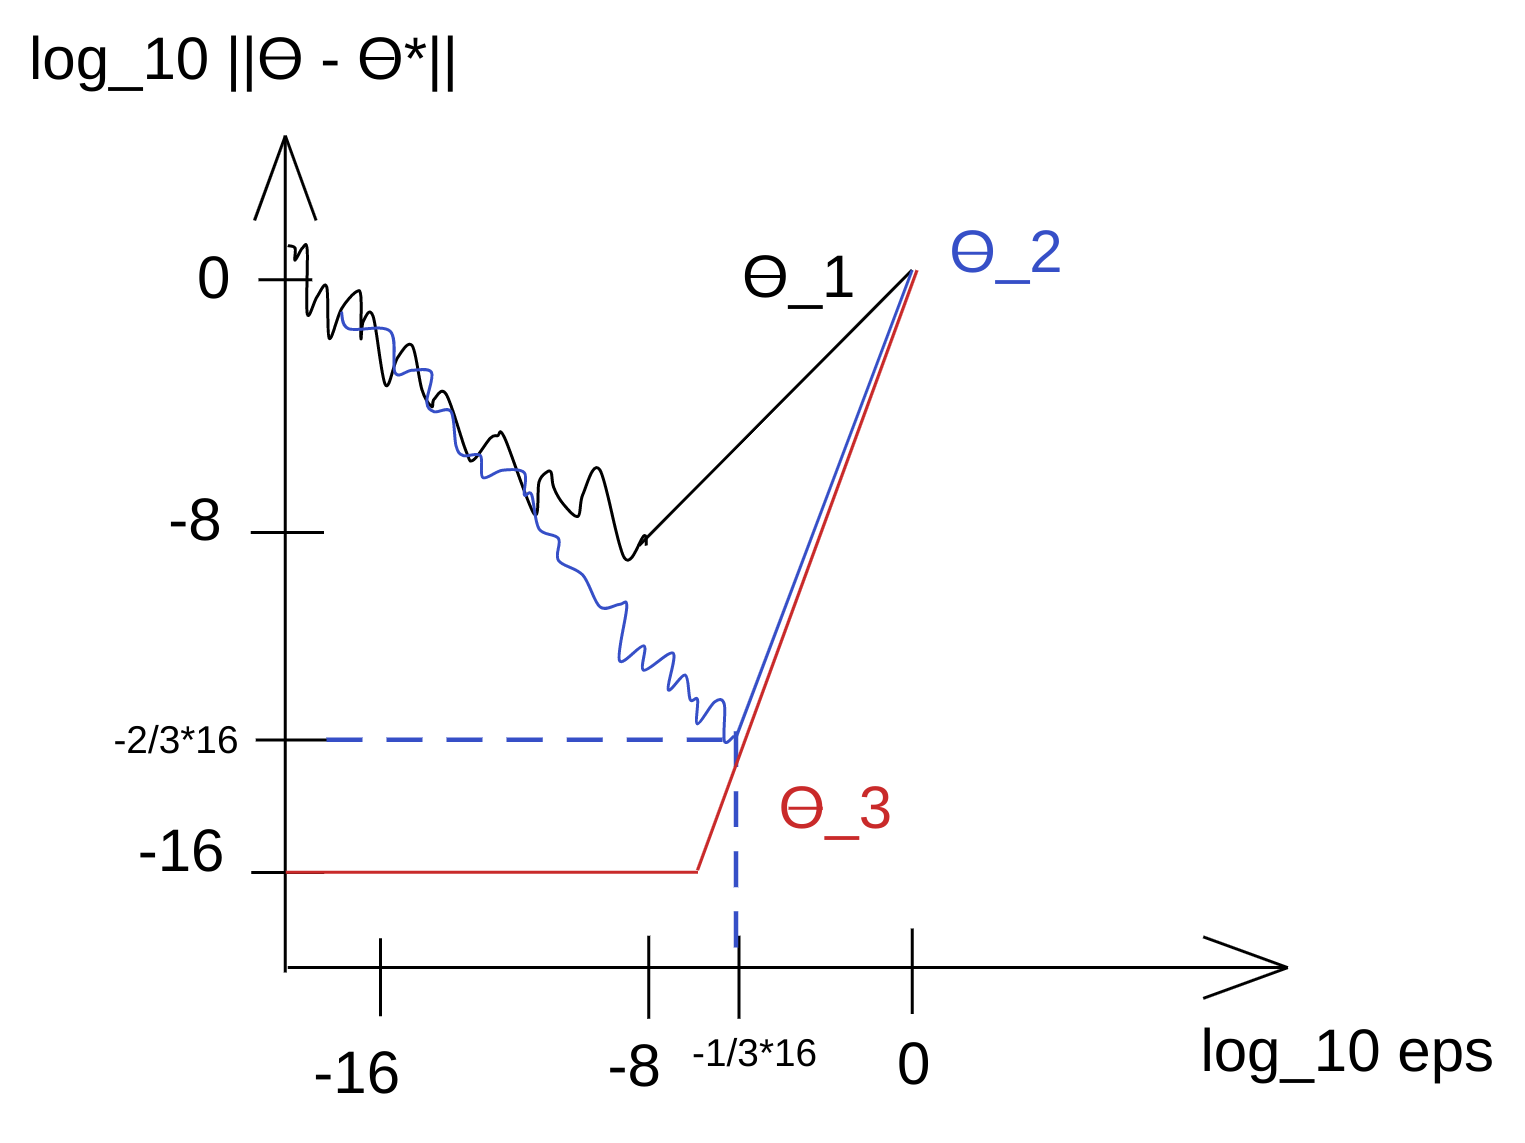
\includegraphics[width=10cm, height=8cm]{images/kir_pic.png}
    \label{ris:im225}
    \caption{Точность при разностном дифференцировании}
\end{figure}
На графике $\Theta_* = \nabla^2 f(x)d$
\\

\textbf{Итого}: 1) способ вычисляет всего 1 градиент, но может получить не такую большую точность. 2) способ считает 2 градиента, но получает лучше точность. 3) способ считает 1 градиент(но из-за перехода к комплексным на самом деле больше), но имеет лучшую сколь угодно низкую точность, применим не ко всем функциям.

